\documentclass{deliverablereport}

\usepackage[style=alphabetic,backend=bibtex]{biblatex}
\addbibresource{../../lib/kbibs/kwarcpubs.bib}
\addbibresource{../../lib/kbibs/extpubs.bib}
\addbibresource{../../lib/kbibs/kwarccrossrefs.bib}
\addbibresource{../../lib/kbibs/extcrossrefs.bib}
\addbibresource{../../lib/deliverables.bib}
%\addbibresource{../../lib/publications.bib}
\addbibresource{rest.bib}
% temporary fix due to http://tex.stackexchange.com/questions/311426/bibliography-error-use-of-blxbblverbaddi-doesnt-match-its-definition-ve
\makeatletter\def\blx@maxline{77}\makeatother

\deliverable{UI}{jupyter-test}
\deliverydate{02/27/2017}
\duedate{02/27/2017 (Month 18)}
\def\pn{OpenDreamKit}
\author{Martin Sandve Aln\ae{}s \& Hans Fangohr \& Vidar Fauske \& Thomas Kluyver \& Benjamin Ragan-Kelley \& MORE?}

\begin{document}
\maketitle
%  Work Package WP6 develops a novel, foundational, knowledge-based framework for
  interfacing existing open source mathematical software systems and knowledge bases into
  a mathematical VRE, where systems can delegate functionalities among each other
  seamlessly without losing semantics.

  The overall Math-in-the-Middle (MitM) Framework developed in WP6 over the last three
  years is described in D6.5; this Report complements it by describing the curated
  contents Math-in-the-Middle (MitM) Ontology which serves as a reference and pivotal
  point for translations between the various input languages of mathematical software
  systems and knowledge bases.

  In a nutshell, the MitM Ontology describes the mathematical objects, concepts, and their
  relations in a general, system-agnostic way in an OMDoc/MMT theory graph while the
  mathematical systems export API theories that describe the system interface language in
  terms of types, classes, constructors, and functions -- again in OMDoc/MMT. These two
  levels of descriptions are linked by OMDoc/MMT alignments that allow the translation of
  expressions between systems.

%%% Local Variables:
%%% mode: visual-line
%%% fill-column: 5000
%%% mode: latex 
%%% TeX-master: "report"
%%% End:

\strut\githubissuedescription
\newpage\tableofcontents\newpage

\newcommand{\nbval}{\texttt{nbval} }

\section{Background on validation} % (fold)

Jupyter notebook documents have become an important part of the development and communication of computational ideas.
While these documents contain code and the output produced by running that code,
they do not guarantee that the code remains valid in changing circumstances or that it continues to function after updates to underlying packages.
These are common problems in all software, but existing testing frameworks do not support notebooks.
Further, Jupyter notebooks aim to be a tool for enabling reproducible computation and communication,
and the ability to validate and verify the contents of notebooks is critical to that goal.
For these reasons, it is important that notebooks can be tested efficiently,
so that authors and readers alike can verify that the notebooks contents remain valid.

The nature of notebooks presents different opportunities and challenges from conventional code testing.
Notebooks are narrative documents, and their code is often not arranged in functions and classes, which normally form the units of code to be tested.
However, because outputs are stored in the notebook,
output from running the code can be compared against previously saved output.

\section{Validating notebooks with \nbval} % (fold)

\begin{figure}[ht]
  \centering
  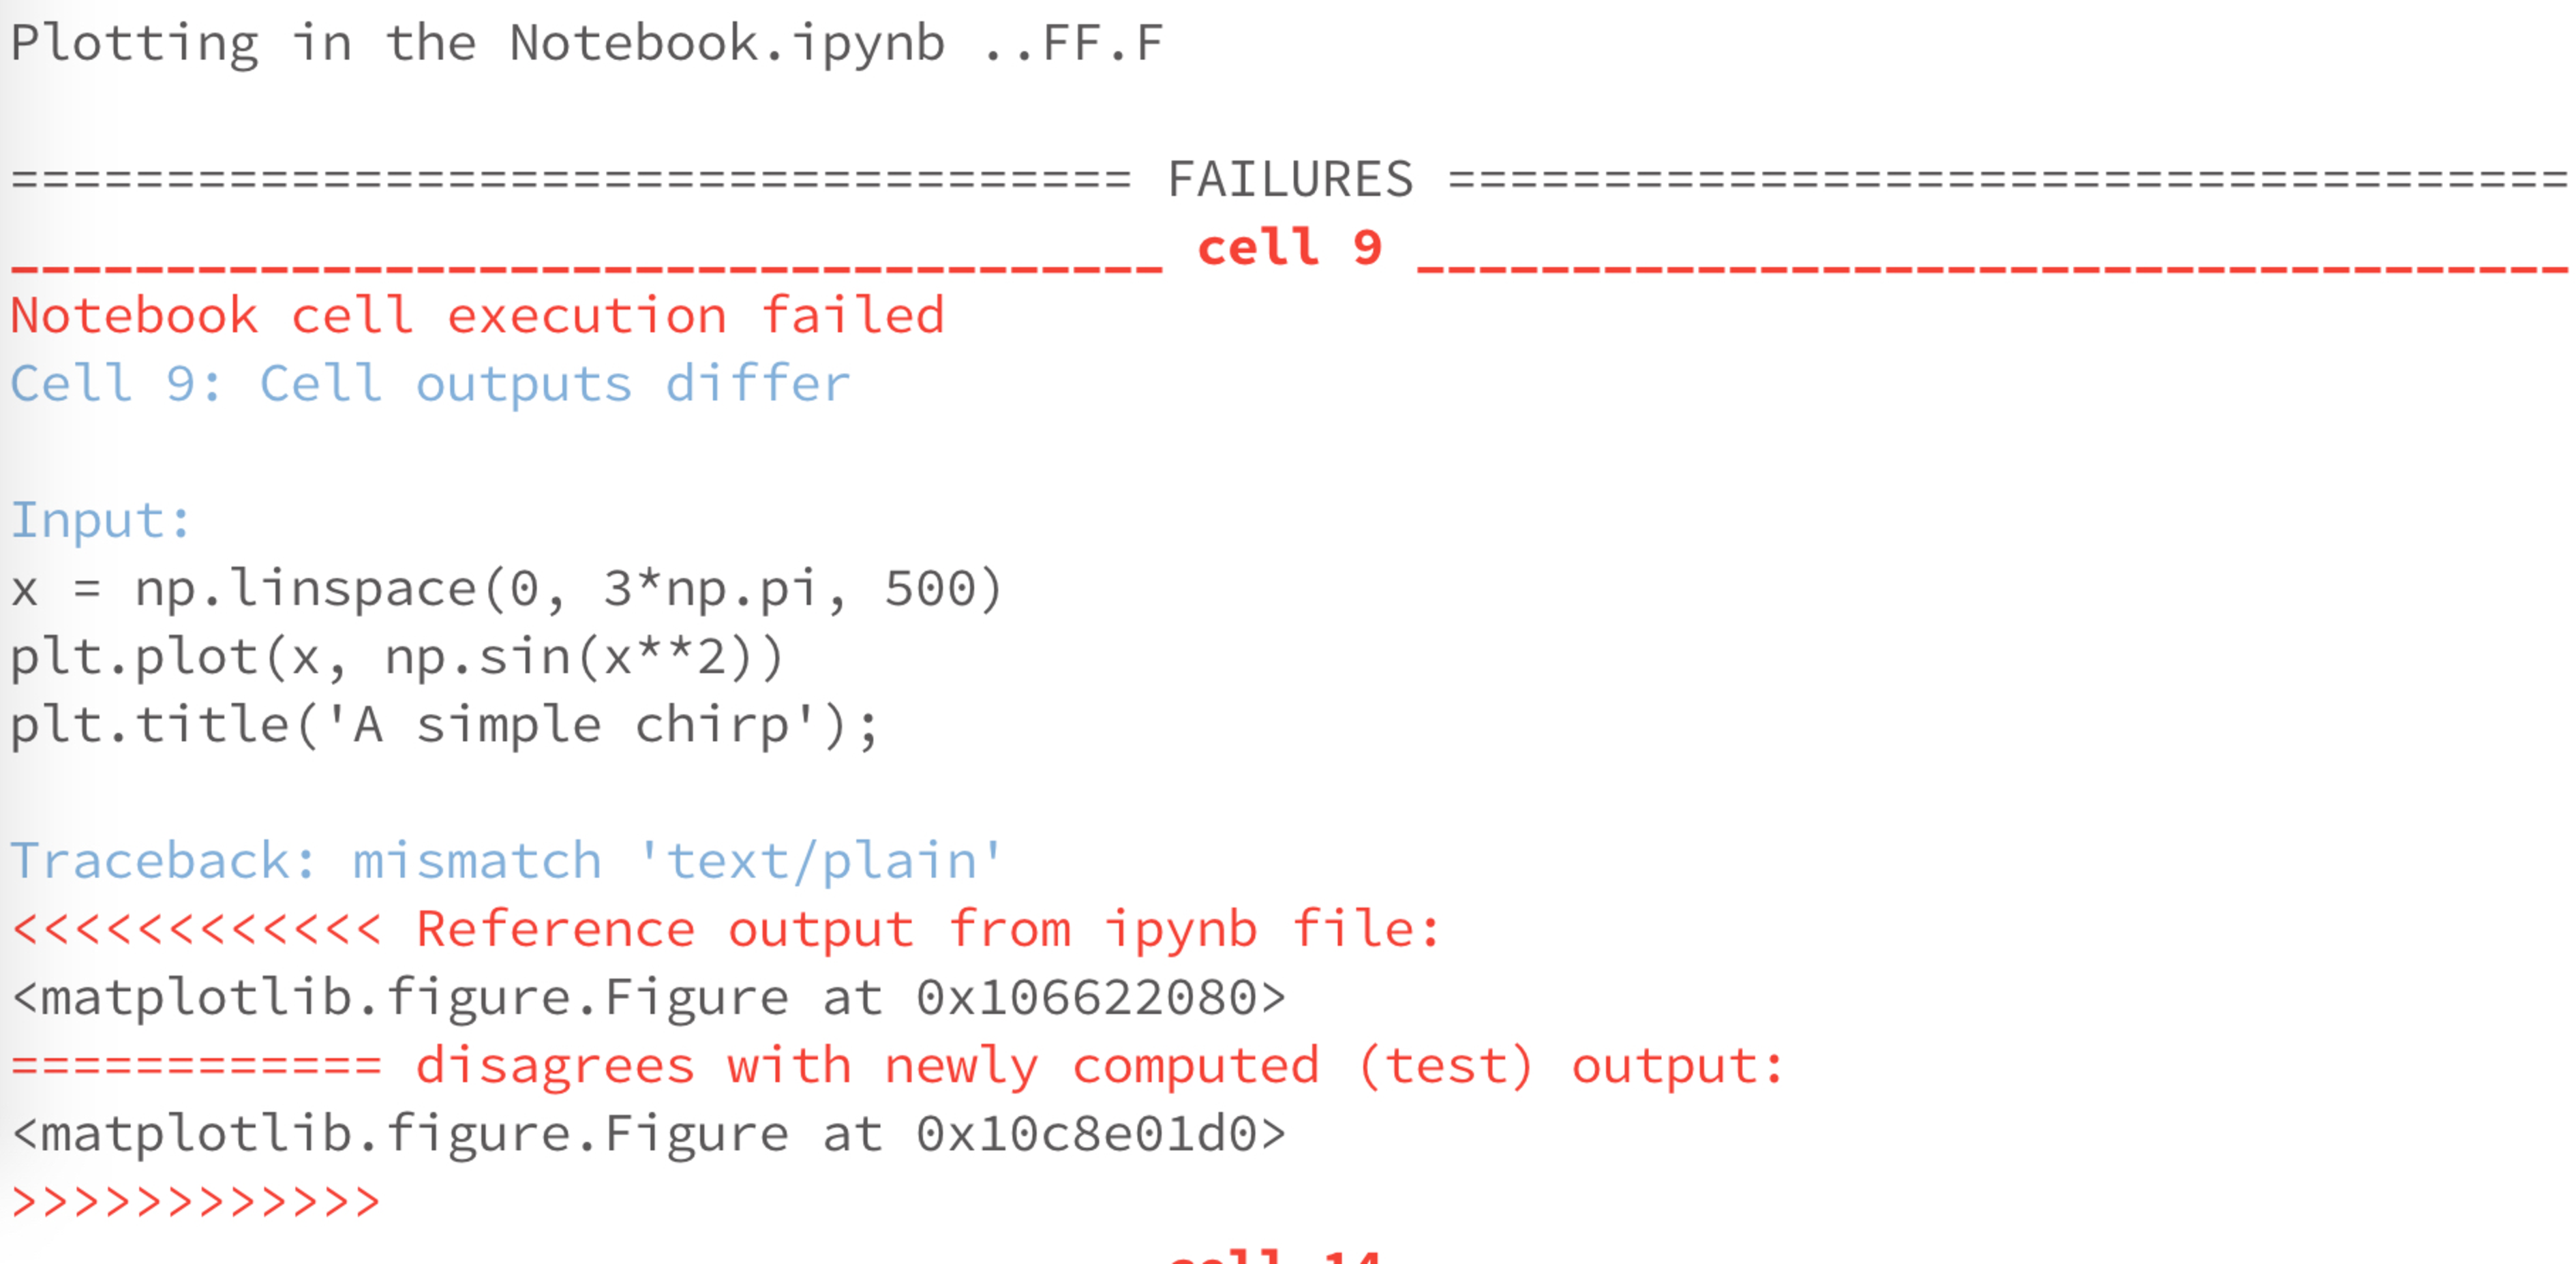
\includegraphics[width=.7\textwidth]{img/nbval-terminal}
  \caption{\nbval output, showing that output changed.}\label{fig:nbval}
\end{figure}

\nbval (\url{https://github.com/computationalmodelling/nbval}) is a new tool for testing notebooks, built as a plugin for the pytest testing framework (\url{http://pytest.org}).
By leveraging existing tools,
\nbval fits well into the software development tools such as continuous integration services and testing environments.

When \nbval encounters a notebook to test, it identifies the language of the notebook from the notebook's metadata and starts a process to run the code found in notebook, called the Kernel.
\nbval communicates with this Kernel via the Jupyter protocol, as in the notebook environment.
Each cell in a notebook constitutes a test, and is executed in order,
as if the notebook had been executed in the interactive notebook environment.

Unlike traditional source code files,
notebooks contain both code to execute and the output.
Validating notebooks can take the output into account or not.
At its most basic level, called `lax mode', \nbval executes a cell, only checking for errors.
This verifies that execution of a notebook completes without error,
but makes no effort to guarantee that the result is the same across executions.

\nbval's default mode is to record the output produced by executing the notebook,
and compare it with the output stored in the notebook.
At its strictest, any visible change in the output will result in a failed test.
Many times, output can contain transient values that are not informative,
such as memory addresses or dates.
To deal with this, \nbval provides an extensible mechanism for normalizing output,
so that these transient values may be excluded from the comparison.

The output checking in \nbval may be controlled on a cell-by-cell basis:
notebook authors may either start with no output checking (`lax mode') and mark specific cells whose output should be checked,
or start with full output checking and mark cells whose output should be ignored.
The author indicate that nbval should not execute a cell at all,
or that it an error is the expected result of a cell.

\section{nbval and reproducibility} % (fold)

\nbval facilitates integrating notebooks into a reproducible scientific workflow.
Tests are integral to maintaining and verifying software,
which is critical for validating and reproducing scientific computation.
A publication can include a notebook that produces its results or figures.
By using \nbval, the validation of this notebook and output can be automated,
to make it more convenient, and thus more likely,
for scientific publications to follow reproducible practices.


\section{nbval and nbdime} % (fold)

Testing notebooks with \nbval involves comparing the notebook as saved,
and the notebook recently run.
This is comparing two notebooks,
which can build on earlier OpenDreamKit work.
\nbval can use nbdime, produced in \delivref{UI}{jupyter-collab},
to display the difference between the before and after notebooks,
for more effective comparison and identification of changes.

\begin{figure}[ht]
  \centering
  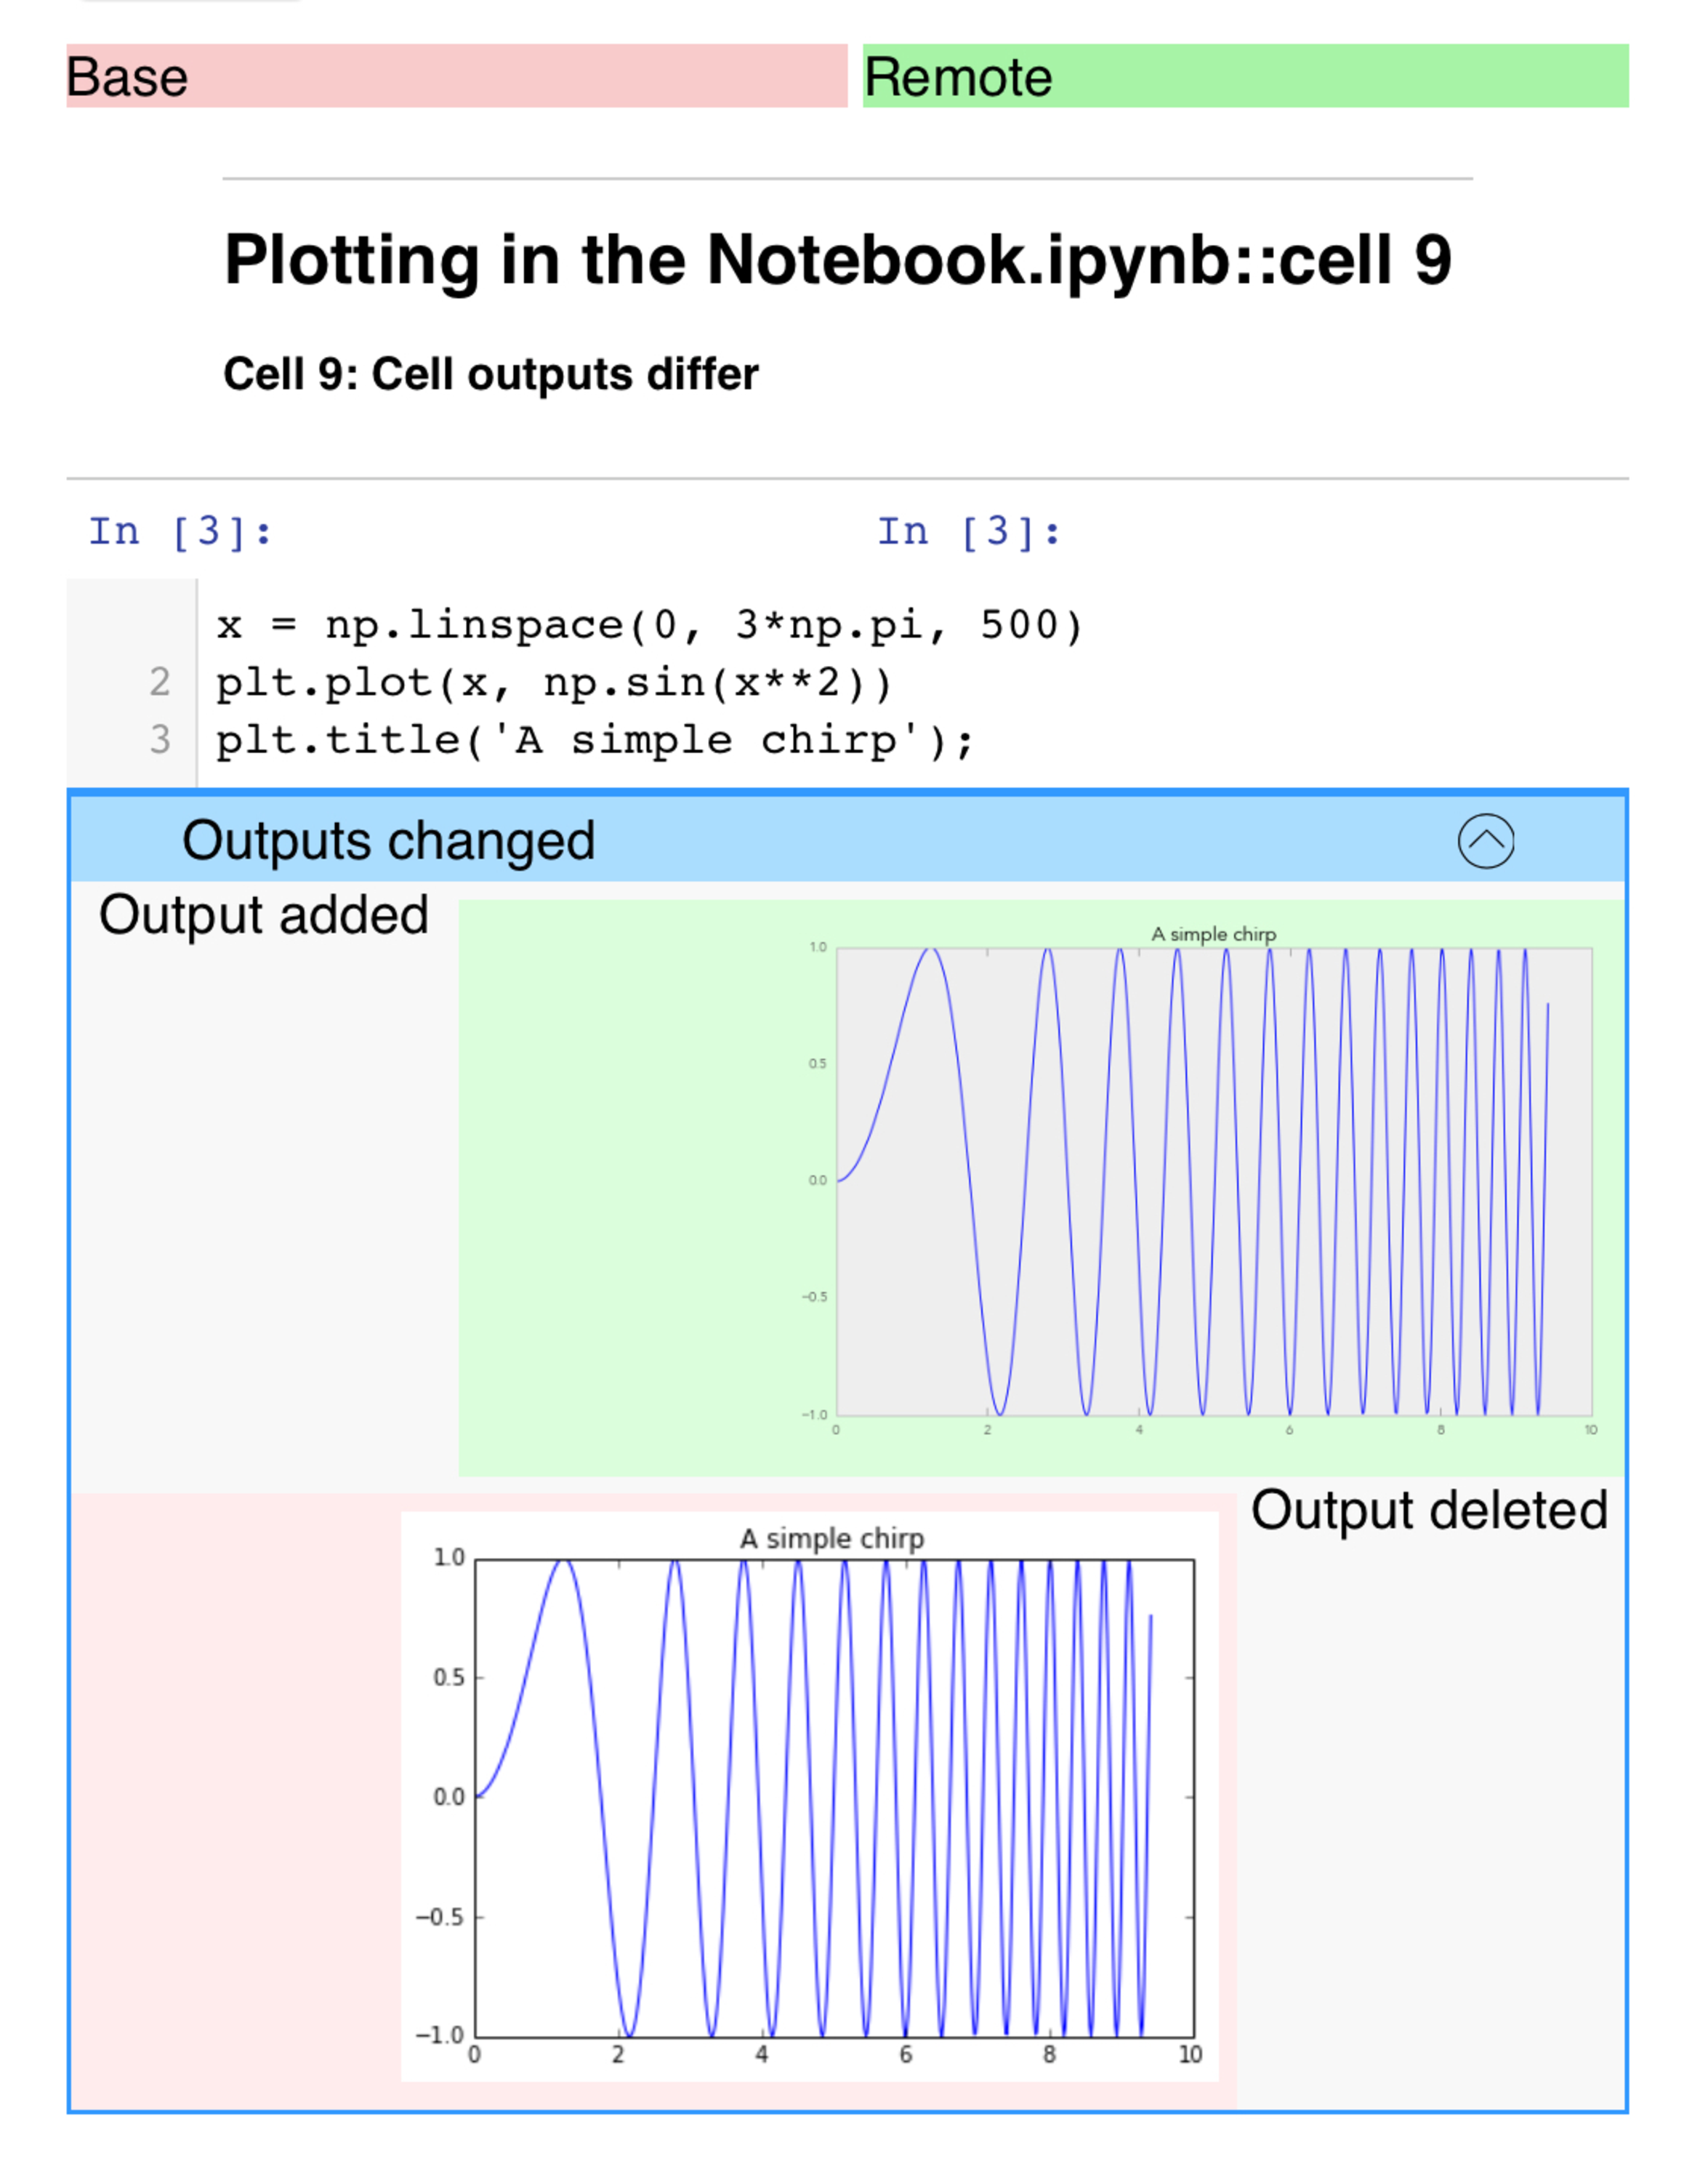
\includegraphics[width=.7\textwidth]{img/nbval-nbdime}
  \caption{An \nbval output rendered with nbdime}\label{fig:nbval-nbdime}
\end{figure}

\section{Future work} % (fold)

\nbval has been integrated successfully into some repositories of notebook-based educational materials and software documentation by OpenDreamKit participants,
and is being integrated into the existing notebook-based documentation of projects in the wider Jupyter community.
We will work to encourage adoption of \nbval for verifying documentation,
and would like to see nbval used to enable verification of scientific publications
now that it has proved its effectiveness in educational materials.

\printbibliography
\end{document}

%%% Local Variables:
%%% mode: latex
%%% TeX-master: t
%%% End:

%  LocalWords:  githubissuedescription newpage tableofcontents newpage printbibliography
